\section{\label{sec:detectors}Detector Geometries}


\subsection{\label{subsec:mono}Monolithic / Single-Volume}

Because of Double CHOOZ's success as mentioned above, we have chosen it as a basis for comparison in this study.
In Chooz and \dc, as well as other major antineutrino experiments such as RENO~\cite{Ahn:2010vy} and Daya Bay~\cite{DayaBay:2012aa}, all of the target material is arranged in a single, central volume. We will hereafter refer to this basic design as the ``monolithic'' type.
This volume is usually arranged in a simple geometric shape such as a sphere, cube, or (as in the \dc\ case) cylinder. Choosing such highly-symmetric configurations simplifies reconstruction of the interaction locations.

% process
In a monolithic detector such as \dc, the prompt and delayed events take place in a single, continuous volume which is large compared to the distance traveled by the neutron. % well, typically they do, and typically it is
% In a real detector, the positions of the positron and neutron events are then reconstructed using the relative time and / or charge registered by the \pmts\ which are spread over the surface of the volume. 
The positions of the positron and neutron events are then reconstructed using the relative time and / or charge registered by \pmts\ (not pictured), which are spread over the surface of the volume. 

% diagram
The version of this geometry that was implemented in our \mc\ simulation is shown in Fig.~\ref{fig:geo_dc}.%, along with a typical d_n0 for scale!
\begin{figure}[ht]
  \begin{center}
    \begin{overpic}[width=0.8\linewidth]%,grid,tics=5]
    {figures/dc_geo_plain_white.eps}
    \linethickness{2pt}
    \put(26,83){\line(1,0){62}}
    \put(54,85){5~m}
    \put(22,12){\line(0,1){62}}
    \put(11,45){5~m}
  \end{overpic}
 %\includegraphics[width=0.8\linewidth]{figures/geo_dc.png}
  \caption{Simulated Double-CHOOZ Geometry   This needs to be replaced by a better figure indicating PMTs around the outside.}
  \label{fig:geo_dc}
  \end{center}
\end{figure}


\subsection{\label{subsec:seg}Segmented}

A key limitation of the monolithic approach is a spatial resolution which is typically considerably larger than the neutron-displacement distance. Stated another way, the goal \dash a measurement of the neutron's displacement \dash depends on determining the difference between the peaks of two closely-overlapping Gaussian curves (i.e., per spatial dimension).
This means that the most immediate factor limiting a monolithic detector's directional capability is its spatial resolution.
The basic concept behind the segmented approach is to improve the spatial resolution by dividing the target volume into a lattice of cells smaller than the desired distance measurement.
% \begin{equation} \label{eq:res_problem}
%   P\ =\ 1/3 \, \left( \sigma_x + \sigma_y + \sigma_z \right)\ >\ d_n,\  \text{where}
% \end{equation}   
% \begin{equation}
%   d_n\ =\ \sqrt{\Delta x^2 + \Delta y^2 + \Delta z^2},\ \text{where}
% \end{equation}
% \begin{equation}
%   \Delta x\ =\ x_{\text{final}} - x_{\text{initial}},\ \text{etc.}
% \end{equation}

% photo
\begin{figure}
  \begin{center}
    % \begin{overpic}[width=0.75\linewidth]{figures/ROL_plain_white.png}
    \begin{overpic}[width=0.7\linewidth]{figures/ROL_plain_white.png}
      \put(-10.0, 50.0){\color{gray} \sffamily $\sim\mathrm{15~cm}$}
    \end{overpic}
      \caption{Photo of ROL $5^3$ demonstrator with TIR behavior visible~\cite{Lane:2015alq}}
      \label{fig:rol}
  \end{center}
\end{figure}

For our example segmented design, we chose the \nl\ detector (Fig.\ref{fig:rol}), in which the target volume is a cube subdivided into cubical cells.
Interaction positions can then be determined to a resolution corresponding to the size of the cell.
The trick then lies in identifying which cell is active at a particular time.
% \nl\ accomplishes this by employing total internal reflection (Fig.~\ref{fig:tir}) to create what is known as a \rol, as shown in Fig.~\ref{fig:rol}.
\nl\ accomplishes this by employing \tir\ to create what is known as a \rol.
In a \rol, light is channeled along each of the three principal axes from the originating cell to the outer faces, which would be instrumented with \pmts.
Combining the information from each face reveals the $\{x,y,z\}$ of the originating cell.

% diagram
\begin{figure}
  \begin{center}
      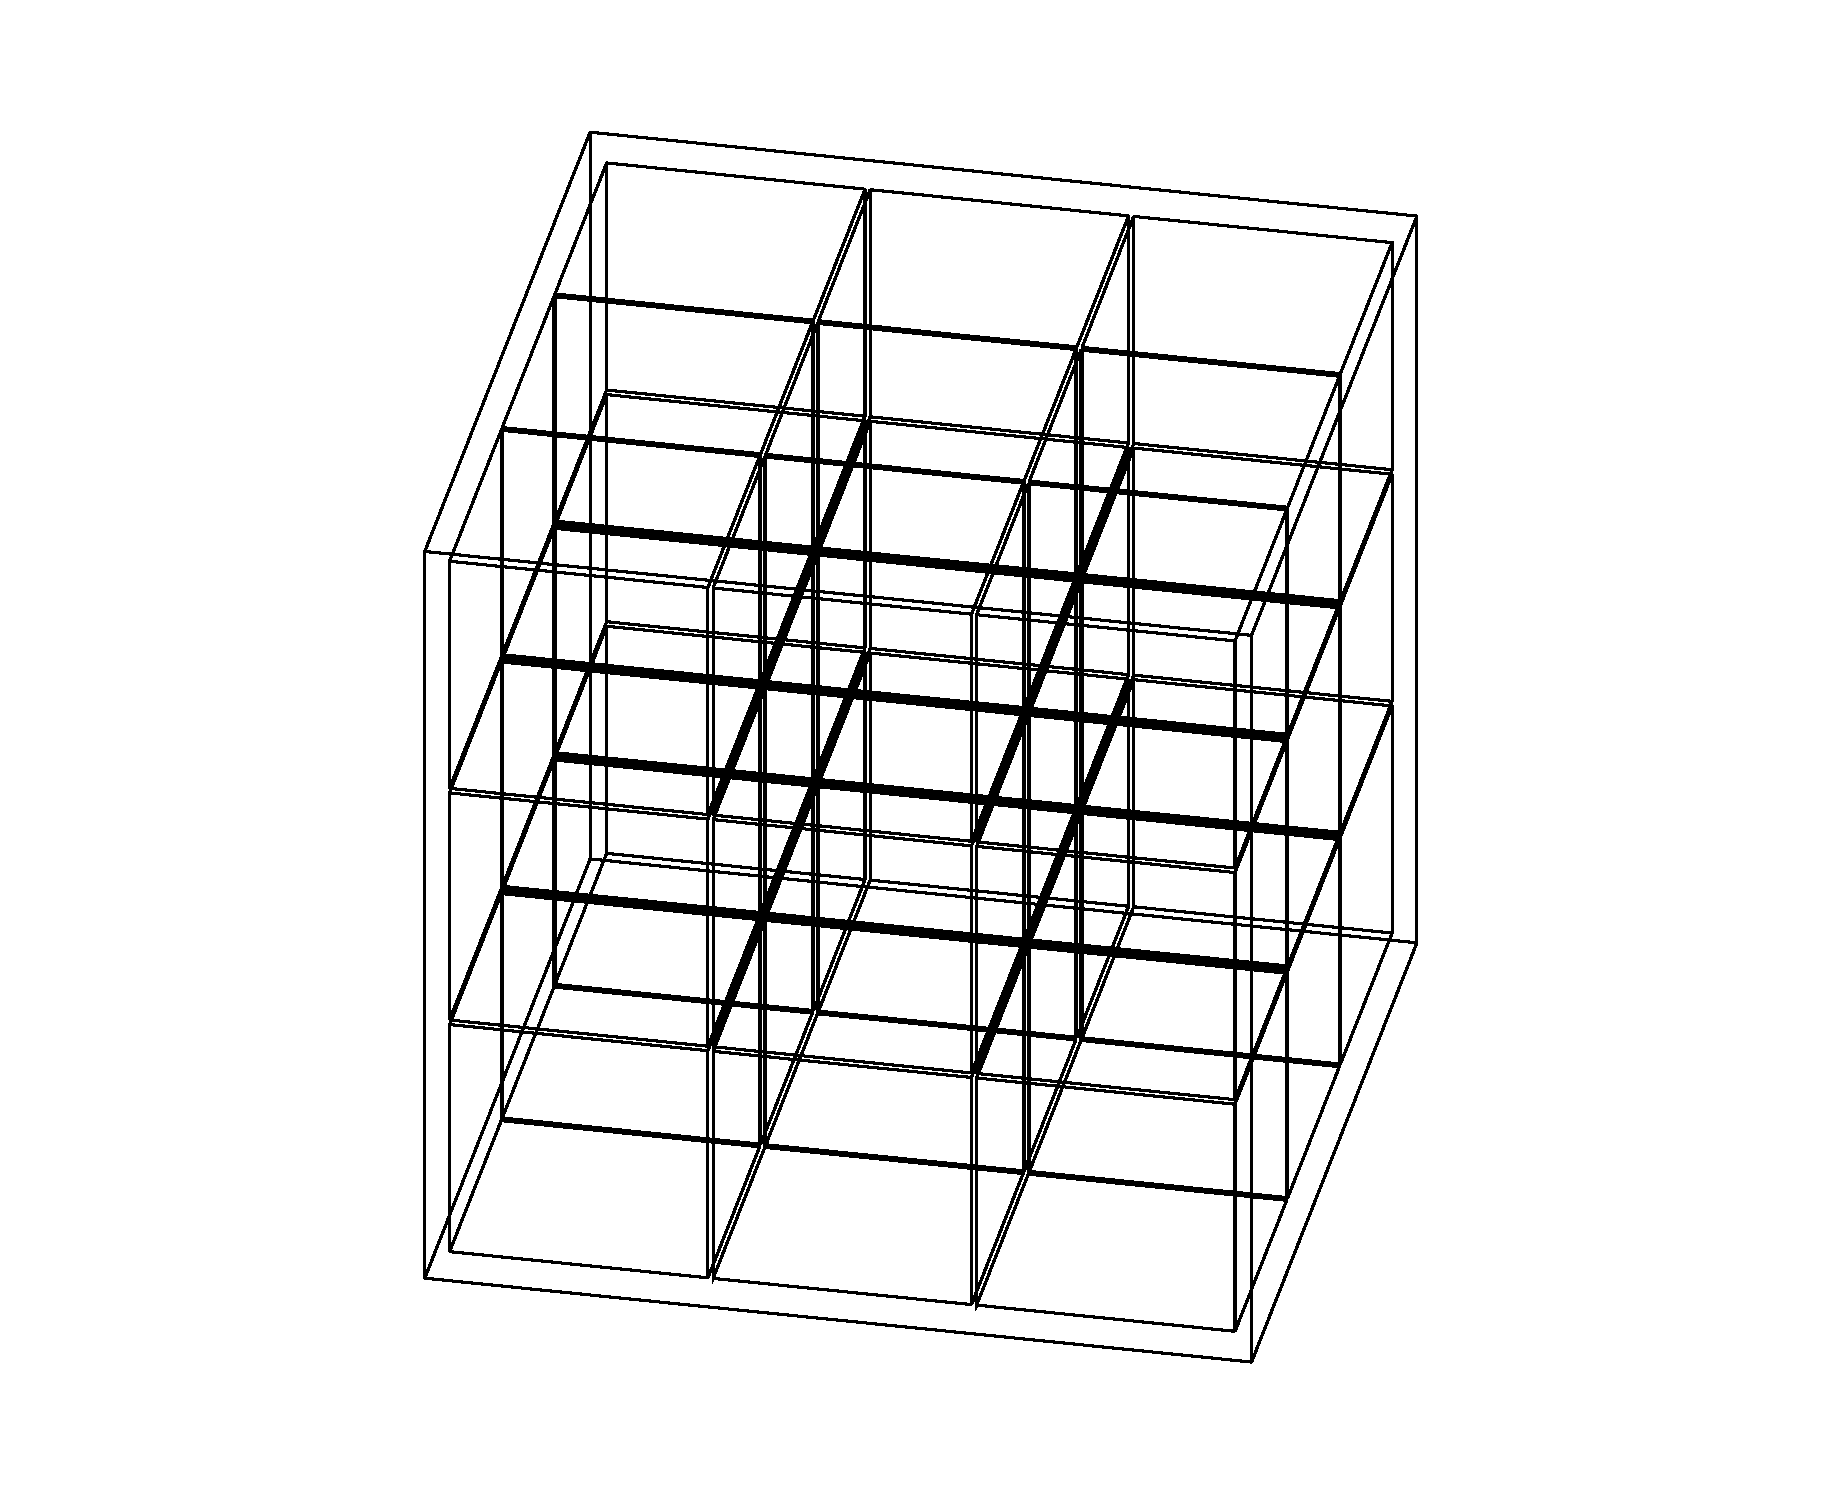
\includegraphics[width=0.7\linewidth]{figures/nulat_geo_scale}
      \caption{Photo of ROL $5^3$ demonstrator with TIR behavior visible~\cite{Lane:2015alq}}
      \label{fig:nl_geo}
  \end{center}
\end{figure}

Directional information from \ibd\ interactions comes from events in which the prompt and delayed events occur in different cells; the direction is then simply a vector from the center of the first cell to the center of the second.
This also indicates that the cell dimensions should be comparable to the typical neutron travel distance in the target material; for this study, the cells were 5-cm cubes.
The simplest configuration, $3 \times 3 \times 3$, gives 1 central cell with a neighbor in every direction; this is the configuration used in our \mc\ simulations and is shown in Fig.~\ref{fig:nl_geo}.
The \nl\ demonstrator currently under construction is $5 \times 5 \times 5$, and the actual NuLat is planned for $15 \times 15 \times 15$~\cite{Lane:2015alq}.\\
\textit{Note: The scintillator cubes in the \rol\ demonstrator in the photograph are $\sim\nicefrac{1}{2}$ the size of those used in NuLat itself and in our simulations, hence the difference in size between the $5^3$ arrays shown in Figs.~\ref{fig:rol}~and~\ref{fig:nl_geo}.}

%\emph{TODO: Add (brief) description of SANDD} %TODO
\subsection{\label{subsec:SANDD}SANDD}

Another segmented detector design was SANDD, a small (6.4 liter) Li-doped pulse shape-sensitive plastic scintillator array, built at LLNL for exploring near-field reactor monitoring, including sensitivity to IBD neutrino direction. (reference to arXiv:2105.00083, Sutanto, et al). The core concept was to use an 8x8 bundle of square lithium doped scintillating rods (5.4 mm x 5.4 mm x 40.64 cm) to detect both the initial interaction and the neutron capture. The configuration is quite similar to a Double Scatter Neutrino Camera built and tested at UH, as part of the program to study a Single Volume Scatter Camera for neutron direction determination, hosted by Livermore SANDIA. 
The inner core of rods was surrounded by two layers of square 2.54cm scintillating rods to tag backgrounds. This prototype worked quite well but needs enlarging to a fiducial volume of order one ton to have enough sensitivity for useful observations near a reactor. 
These experiments demonstrate the viability of utilizing a bundle of scintillating rods for an IBD sensor, but also highlight the problem of requiring many detector and electronics channels (~40,000) when scaling up to the needed fiducial volumes for reactor studies, even from a few meters distance. 

\subsection{\label{subsec:sep}Separation}

% the (neutron-) Neutron-scattering problem
\subsubsection{\label{subsubsec:scat}The Neutron-Scattering Problem}

% \begin{sidewaysfigure}[ht]
%\begin{figure}[ht]
\begin{figure*}[ht]
  \centering
    \begin{overpic}[width=0.48\linewidth]{figures/scattering_positions.png}
    \textbf{\textit{(a)}} % subfigure label -- manual for now
    \put(10.0, 85.0){\sffamily \large \color{orange} 2}
    \put(60.0, 85.0){\sffamily \large \color{orange} 5}
    \put(10.0, 35.0){\sffamily \large \color{orange} 10}
    \put(60.0, 35.0){\sffamily \large \color{orange} 20}
  \end{overpic}
  %\rule{0.7\linewidth}{0.5pt}
  \unskip\ \vrule\ 
  \begin{overpic}[width=0.48\linewidth]{figures/scattering_cosines.png}
    \textbf{\textit{(b)}} % subfigure label -- manual for now
    \put(10.0, 85.0){\sffamily \large \color{orange} 2}
    \put(60.0, 85.0){\sffamily \large \color{orange} 5}
    \put(10.0, 35.0){\sffamily \large \color{orange} 10}
    \put(60.0, 35.0){\sffamily \large \color{orange} 20}
  \end{overpic}
  \caption{\textit{(a)} Displacements and \textit{(b)} corresponding cosines (vs. initial direction) for a uniform beam of 10-keV neutrons undergoing scattering and thermalization in plastic scintillator.}
  \label{fig:santa_scatbad}
% \end{sidewaysfigure}
%\end{figure}
\end{figure*}

A fundamental challenge for any $\bar{\nu_e}$ \ibd\ detector is that neutron scattering quickly degrades directionality. Fig.~\ref{fig:santa_scatbad} depicts the positions of neutrons after 2, 5, 10, and 20 scatters.
The first panel represents an overhead view of neutrons scattering in target material after being given an (identical) initial velocity in the upward direction. After the first scatter, the distribution is quite clearly forward-biased, but it spreads out considerably in just a few more scatters. After 20 scatters \dash a typical total \dash the distribution is only slightly heavier in positive $z$ than in negative $z$, and the transverse spread is comparable to the forward-backward spread.
The second panel of Fig.~\ref{fig:santa_scatbad} shows a quantitative view of this process, representing the overall directional information by the distribution  of $\mathrm{Cos}(\psi)$ at each step. In $N=2$, the momenta are strongly concentrated in a narrow cone about the initial momentum, but in $N=5$, the cone is considerably broader and much less sharply-defined. The stark contrast between $N=2$ and $N=5$ indicates how detrimental even a few scatters are to the directional information carried by the neutron. By the time the neutron captures at around $N=20$, the trend in $\mathrm{Cos}(\psi)$ is quite weak.

The problem this causes in reconstructing the direction of the original incident \nb\ is that the position distributions in $\{x,y,z\}$ of the prompt and delayed events become a pair of closely-overlapping Gaussians, both having standard deviations that are considerably larger than the separation between their means.
This indicates that improving the position resolution $P$ of a traditional \ibd\ detector can only increase its directional capability up to the point at which $P \sim d_{n}$, the typical neutron-capture distance ($\sim10^0$~cm in the relevant materials).
At this point, the neutron-scattering process becomes the dominating factor limiting improvements in the detector's angular resolution.

% the SANTA soln.
\subsubsection{\label{subsubsec:santa_sln}The SANTA Solution}

% concept fig.
% \begin{sidewaysfigure}[ht]
\begin{figure}[ht]
  \begin{center}
   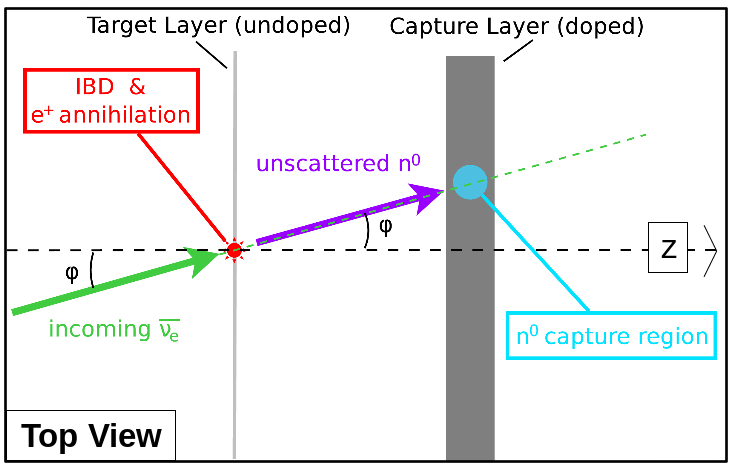
\includegraphics[width=0.8\linewidth]{figures/santa_concept}
   \caption{Segmented Detection Concept}
   \label{fig:santa_concept}
  \end{center}
% \end{sidewaysfigure}
\end{figure}

The loss of directional information due to neutron scattering is an inherent limitation in bulk-volume detectors, whether they are monolithic like \dc\ or subdivided like \nl. %\
One proposed solution to this problem is the \santa~\cite{Safdi:2014hwa}, which allows the neutron to travel a long distance in its original direction before its first scatter. This requires the neutron to leave the target material almost immediately after it is produced, then travel some relatively long distance, then enter a second volume of target material and be captured there. As shown in Fig.~\ref{fig:santa_concept}, \santa\ proposes to achieve this by arranging the target material into two separate layers: a very thin ``target'' layer for the prompt event and neutron production, and a thicker ``capture'' layer for neutron thermalization and capture. In order to encourage the neutron to capture in the correct layer, the target layer would not be doped with any neutron-capture agents, and the capture layer would be doped rather heavily.

% geometry --- overall
\begin{figure}[ht]
  \begin{center}
%   \includegraphics[width=0.8\linewidth]{figures/santa_geo.png}
    \begin{overpic}[width=0.7\linewidth]%,grid,tics=5]
      {figures/santa_plain_axes.png}
      \linethickness{2pt}
      \put(23.5,10){\line(1,-0.13){22.75}}
      \put(30,4){1~m}
      \put(47,6.9){\line(1,0.62){21.4}}
      \put(63,10){2~m}
      \put(69,20.8){\line(0,1){50}}
      \put(73,45){2~m}
      \put(-12,60){\scriptsize Capture Plane:}
      \put(-12,56){\scriptsize Doped, 6~cm thick}
      \put(-12,40){\scriptsize Both planes:}
      \put(-12,36){\scriptsize 40 bars @ 5~cm tall}
      \put(72,70){\scriptsize Target Plane:}
      \put(72,66){\scriptsize Undoped,}
      \put(72,62){\scriptsize 0.5~cm thick}
    \end{overpic}
  \caption{Simulated \santa\ Geometry}
  \label{fig:santa_geo}
  \end{center}
\end{figure}

The implementation of \santa\ used in this MC study was based on a possible realization proposed in~\cite{Safdi:2014hwa}. It contains a 0.5-cm-thick undoped target layer separated by 1~m from a 6-cm-thick capture layer doped at 5\%wt~natural~B, as shown in Fig.~\ref{fig:santa_geo}. Both layers are composed of EJ-254 plastic scintillator and are 2~m square.
No explicit mechanism was proposed by~\cite{Safdi:2014hwa} for measuring the locations of the interactions in the scintillator. For this study, the layers were subdivided into a stack of optically-separated horizontal bars of height 5~cm and separation 0.1~cm. In a real detector, \pmts\ would then be placed at either end of each bar.
For typical interactions (both prompt and delayed), a strong signal will be produced in exactly one bar; this gives the vertical position. Horizontal position could be determined by comparing light output at either end. If fast-timing measurements are available, this position determination could be enhanced by comparing photon arrival times at either end.
% An end-on cross-sectional view of the bars and optical separators is shown in Fig.~\ref{fig:santa_geo_closeup}.

A possible detector featuring the \santa\ geometry is shown in Fig.~\ref{fig:santa_geo}.
This is the arrangement used in all simulations discussed below.
This version is based on the configuration proposed in~\cite{Safdi:2014hwa}: a pair of $2 \times 2~\mathrm{m}^{2}$ planes, separated by a 1-m gap.
At \uh, we took this concept and considered how it might be realized in an actual detector.
To this end, we subdivided each plane into a set of 40 scintillator bars, each 50~mm tall and separated by 1~mm from the next bar.
Furthermore, we inserted a 0.5-mm strip of black acrylic for optical separation between each bar.
This setup would be completed by coupling a 2-inch \pmt\ or \sipm\ to either end of each bar, for 160 optical detectors total (not pictured for clarity).
This way, the positions of scintillation events could be measured as follows:
\begin{itemize}
  \item $x$ coordinate: relative total charge at either end of scintillating bar
  \item $y$ coordinate: center of scintillating bar
  \item $z$ coordinate: center of scintillating plane
\end{itemize}


\subsection{\label{subsec:hyb}Hybrid}

Our collaboration felt that the \santa\ approach featured an ingenious insight on solving the aforementioned neutron-scattering problem; however, we also anticipated some major practical limitations with the design as laid out in the original paper. %~\cite{} again?
Our biggest concerns were that, relative to the more traditional designs:
\begin{enumerate}
  \item The much-larger surface-area-to-volume ratio would expose the detector to severe levels of background noise, especially in our targeted near-surface deployment scenario; and
  \item The much-smaller target-volume-to-footprint ratio would restrict the achievable target mass in any real deployment environment to impractically-small amounts.%\footnote{Recall that the detector only registers \ibd\ interactions taking place in the target plane, so only the slimmer of the two planes contributes to the target mass}. % FIXME: this document class doesn't seem to support footnotes %UPDATE: temporary solution now in place
\end{enumerate}
It is worth noting that the \santa\ design does inherently compensate somewhat for both of these effects. % TODO: elaborate on this?
However, our simulations indicated that this compensation alone would likely be insufficient to make the original design practically viable, as will be discussed in \S\ref{subsec:esim} below.

We therefore set out to devise a class of detector designs that would strike a balance between \santa's directional performance and the more-traditional detectors' larger target mass and stronger resilience against backgrounds.
In this work, we refer to such detector plans as ``hybrid'' designs.
All of them seek to improve directional performance by incorporating space for the neutron to exit the target medium almost immediately after production and then undergo thermalization and capture in a different target segment, which is the driving behavior behind \santa's directional capabilities.

\begin{figure*}[ht]
    \centering
    \begin{overpic}[width=0.48\linewidth,percent]{figures/checkerboard-2d_zoomed_geo_scale.png}
      \put(0.0,75.0){\textit{(a)} Closeup Showing Lattice Arrangement}
      \label{subfig:chkbd_2d_zoomed}
    \end{overpic}
    \unskip\ \vrule\ 
    \begin{overpic}[width=0.48\linewidth,percent]{figures/checkerboard-2d_full_geo_scale.png}
      \put(05.0,75.0){\textit{(b)} Full Array Used in Simulations}
      \label{fig:chkbd_2d_full}
    \end{overpic}
    \caption{2D-Checkerboard Geometry}
    \label{fig:chkbd_2d}
\end{figure*}

\begin{figure*}[ht]
    \centering
    \begin{overpic}[width=0.48\linewidth,percent]{figures/checkerboard-3d_zoomed_geo_scale.png}
      \put(0.0,75.0){\textit{(a)} Closeup Showing Lattice Arrangement}
      \label{subfig:chkbd_3d_zoomed}
    \end{overpic}
    \unskip\ \vrule\ 
    \begin{overpic}[width=0.48\linewidth,percent]{figures/checkerboard-3d_full_geo_scale.png}
      \put(05.0,75.0){\textit{(b)} Full Array Used in Simulations}
      \label{fig:chkbd_3d_full}
    \end{overpic}
    \caption{3D-Checkerboard Geometry}
    \label{fig:chkbd_3d}
\end{figure*}

One of our primary approaches was to provide this free-flight space by simply removing alternating detector segments from the \sandd\- and \nl\-style configurations in a ``checkerboard'' pattern.
This pattern is defined for a 2D (3D) lattice by row, column, and layer number according to the following:
\begin{equation}
    %ROW\ \%\ 2\ ==\ COLUMN\ \%\ 2\ (\ ==\ LAYER\ \%\ 2\ )
    ROW\ \%\ 2\ ==\ COL\ \%\ 2\ (\ ==\ LYR\ \%\ 2\ )
\end{equation}
Renderings of our simulated versions of these arrangements are shown in Figs.~\ref{fig:chkbd_2d} and~\ref{fig:chkbd_3d}.

After investigating these and other geometries, we combined everything we learned and settled on a new design which we propose in this work; it is discussed in detail below in \S\ref{sec:newdesign}.


%% end \section


